\documentclass[a4paper,10pt]{article}
\usepackage[utf8]{inputenc}
\usepackage[T1]{fontenc}
\usepackage[french]{babel}
\usepackage[normalem]{ulem}
\usepackage{geometry}
\usepackage{lmodern}
\usepackage{graphicx}
% \usepackage{setspace}
% \usepackage{titlesec}
\usepackage{geometry}
\usepackage{placeins}
% \usepackage{epsfig}
% \usepackage{hyperref}
% \usepackage{url}
% \usepackage{cite}
% \usepackage{listings}
% \usepackage{xcolor}


%\lstset{
%language=Java,
%basicstyle=\normalsize,
%upquote=true,
%aboveskip={1.5\baselineskip},
%columns=fullflexible,
%showstringspaces=false,
%extendedchars=true,
%breaklines=true,
%showtabs=false,
%showspaces=false,
%showstringspaces=false,
%identifierstyle=\ttfamily,
%keywordstyle=\color[rgb]{0,0,1},
%commentstyle=\color[rgb]{0.133,0.545,0.133},
%stringstyle=\color[rgb]{0.627,0.126,0.941},
%}

\geometry{top=3cm, bottom=3cm, left=2cm, right=2cm}

\title{Rapport\\Architecture Logicielle\\Jeu 2D autour d'un framework\\Année 2015/2016 }
\author{Raphaël Jorel, Antoine Laulan}



\begin{document}


\begin{figure}
    \begin{center}
    \includegraphics[scale=0.7]{images/logo-bdx.pdf}
    \end{center}
\end{figure}
\maketitle




\newpage
\section{Introduction }
Notre jeu a été produit dans le cadre de l'UE architecture logicielle. Le but étant de créer un jeu à l'aide
d'un framework fourni et cela sans modifier celui-ci.
Dans ce rapport nous présenterons notre jeu et nous fournirons une critique du \textit{framework} utilisé. \\

Comme le sujet était libre, nous avons choisi de recréer une copie simplifiée du célèbre jeu Breakout.
Simple en apparence, mais qui nous aura tout de même donné du fil à retordre sur certains aspects
que nous ne soupcionnions pas. Nous dédierons une partie à l'explication de ces problèmes rencontrés.


\section{Firewall Breaker}
\subsection{Présentation}
    Tout d'abord, une petite capture d'écran afin d'apprécier le rendu du jeu et des \textit{assets} qui ont été
    utilisés  :

\FloatBarrier
		\begin{figure}[!h]
    		\begin{center}
	   	  	\includegraphics[scale= 0.5]{images/gameView.png}
          	\caption{Vue du jeu}
    		\end{center}
		\end{figure}
\FloatBarrier

Le joueur contrôle une palette et doit, en faisant rebondir la balle, détruire les briques pour gagner.
Pour se faire il peut être aidé de divers bonus et briques spéciales. La partie s'arrête lorsque le joueur
a détruit toutes les briques qui peuvent l'être, ou lorsque celui-ci n'a plus de vie.

\subsection{Fonctionnalités du jeu}
    \subsubsection{Le joueur}
        Le joueur ne peut faire que deux choses : aller à droite ou à gauche. Il doit rattraper la balle
        qui se déplace pour la relancer dans le jeu et ainsi casser les briques. Comme sus-dit, il pourra
        être aidé par différents bonus, et ainsi augmenter sa capacité de destruction.
	
	\newpage
    \subsubsection{La balle}
        La balle se déplace et rebondit sur les briques, les murs (invisibles sur les côtés) et le joueur.
        Ses rebonds gardent les mêmes angles lorsqu'elle rebondit sur les murs et les briques, mais suivant
        l'endroit où elle touche le joueur, elle gagne ou perd en vitesse.

    \subsubsection{Les briques}
        Il y a quatre sortes de briques :
        \begin{itemize}
            \item les basiques : elles n'ont aucun effet particulier, mis à part le fait de rapporter des points lorsque la balle les détruit,
            \item les indestructibles : elles font barrage à la balle et ne peuvent être détruites,
            \item les briques de bonus : elles déclenchent l'apparition aléatoire de bonus lorsqu'elles sont détruites,
            \item les briques explosives : elles explosent lorsqu'elles rentrent en contact avec la balle et cassent toutes les briques situées autour d'elles 
                    et ceci dans un rayon de taille aléatoire.
        \end{itemize}

        Lorsque toutes les briques sont cassées, le niveau est terminé. Toutes les briques cassables
        ne nécessitent qu'un seul coup pour être détruites.

    \subsubsection{Les bonus}
        Afin de varier un peu le jeu et de coller un peu plus à l'esprit d'un Breakout nous avons intégrer la possibilité au joueur
        d'utiliser des bonus. Ceux-ci ont uniquement un effet "positif" sur la parite du joueur. Voici la liste des bonus mis 
        à la disposition du joueur : 
        \begin{itemize}
            \item \textbf{life Bonus} : représenté par un coeur, caractérisé par le rajout d'une vie supplémentaire,
            \item \textbf{weapon Bonus} : représenté par un pistolet et caractérisé par le tir d'une salve (limitée dans le temps) de balles depuis
            la palette du joueur en direction des briques,
            \item \textbf{bomb Bonus} : représenté par une bombe. Ce bonus à pour effet de transformer une brique restante 
            en brique explosive et de la faire exploser. L'explosion a le comportement d'une brique explosive classique.
            \item \textbf{fireball Bonus} : représenté par une boule de feu. Il provoque un changement d'état temporaire de la balle (\textit{fireball}) 
            qui ne 	rebondit alors plus sur les briques mais passe à travers tout à l'exception des briques indestructibles.
        \end{itemize}

        Chacun de ces bonus est associé à une probabilité, ainsi  par exemple le bonus de vie supplémentaire a moins
        de chance d'apparaître que les autres, car le nombre de vies est un élément cruxial à prendre
        en compte, et que nous ne souhaitons pas que le jeu soit trop facile, cela va de soit.
        Nous proposerons également au joueur l'achat de futurs DLC pour obtenir de nouveaux bonus encore plus dévastateurs..

    \subsubsection{Gestion des parties}
        Il est toujours agréable de pouvoir recommencer une partie, sans etre obligé de relancer un
        programme. Pour cela, la fonctionnalité \textit{new (game)} a été apportée, en plus de la
        possibilité de quitter. Cependant, il est impossible de suspendre une partie et de la reprendre.
        Il faut donc que vous soyez vraiment sûr de ne pas être dérangé et de n'avoir rien besoin de faire pendant vos parties
        (que l'on espérera enflammée, évidemment).


\subsection{Architecture}
    Un bon jeu implique une bonne architecture. L'inverse est moins évidente..
	Nous allons dans cette partie vous présenter l'architecture logicielle de notre jeu. Ceci sera fait à l'aide de
	diagrammes de classes.
	Nous metrons en évidence les connexions entre nos classes et les classes du framework.

	\newpage
	\subsubsection{Diagrammes de classe}

		\FloatBarrier
		\begin{figure}[!h]
    		\begin{center}
	  	  	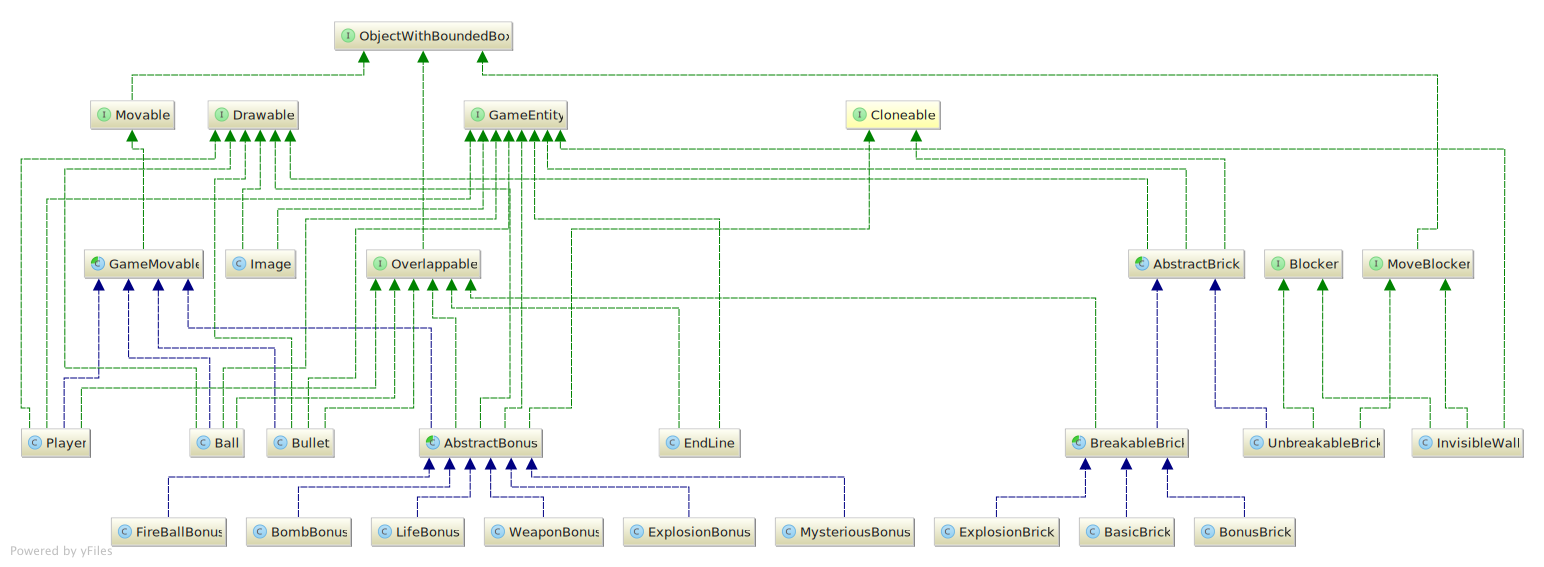
\includegraphics[scale=0.175]{images/whiteEntityDiagram.jpg}
          	\caption{Diagramme de classe des entités}
    		\end{center}
		\end{figure}
		\FloatBarrier
		
		
 		\FloatBarrier
 		\begin{figure}[!h]
     		\begin{center}
 	  	  	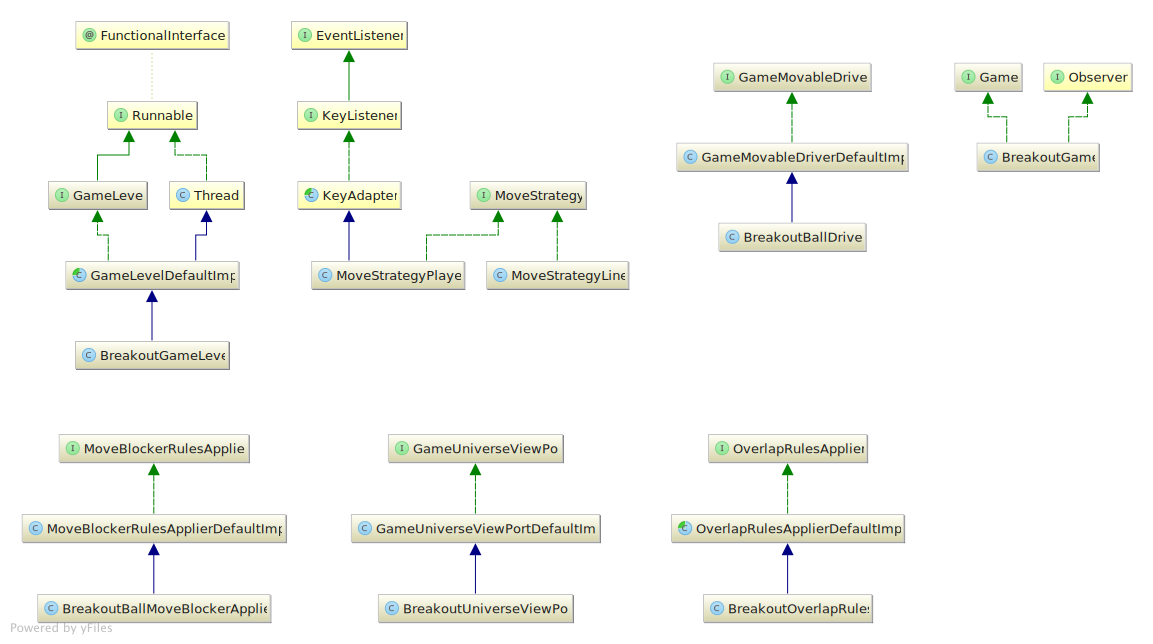
\includegraphics[scale=0.2]{images/whiteSeveralDiagram.jpg}
           	\caption{Multi diagramme de classe}
     		\end{center}
 		\end{figure}
 		\FloatBarrier
 		\paragraph{Description :}
 		Plusieurs classes forment de petits diagrammes de classes. Nous les avons regroupés dans une seule est même image. Pour les différencier
 		nous avons utilisé un code couleur. Ce code couleur est détaillé dans la liste suivante : \\
 		\begin{itemize}
 		\item noir : gestion des levels du jeu,
 		\item rouge : stratégie de déplacement du joueur,
 		\item bleu : driver de la balle,
 		\item vert : gestion de la fenêtre IHM du jeu,
 		\item rose : move blocker pour la belle,
 		\item orange : gestion du fond d'écran,
 		\item bleu ciel : gestion des overlappables.
 		\end{itemize}


\subsection{Implémentation}
    Après cette présentation des fonctionnalités et de l'architecture du jeu, nous allons dans la partie suivante
    parler de son implémentation et donc du travail qui a été effectué.

    \subsubsection{Les niveaux}
        Afin de ne pas avoir à écrire statiquement la configuration des briques d'un niveau, nous avons
        utilisé des fichiers externes, au format \textit{.txt}, pour le faire. Chaque type de brique est représentée par un numéro.
        Théoriquement, il est possible d'avoir un nombre de brique en largeur et en hauteur aussi grand qu'on le souhaite,
        il faut juste préciser cela dans au début du fichier de description, mais pour des raisons de jouabilité, il
        est recommandé de se limiter à des grilles de 16x16. Ainsi, la balle a toujours la place de bouger entre les murs 
        exterieurs et les briques. \\

        Pour éviter d'instancier chaque brique une à une, nous nous sommes servis du \textit{design pattern prototype},
        cela permettant d'avoir les briques de bases dans un tableau et ensuite de les cloner en fonction du
        fichier de description.

    \subsubsection{Stratégies de déplacement}
        Les stratégies permettent de définir comment un objet va se déplacer. Pour notre jeu, nous n'avons eu besoin
        que de deux stratégies  : celle du joueur et celle des autres entités. \\ Les autres entités
        se déplacent verticalement, vers le bas pour les bonus et vers le haut pour les balles de pistolet.
        Le joueur quant à lui bouge suivant l'action de l'utilisateur sur le clavier. Son déplacement est uniquement horizontal.

    \subsubsection{Fenêtre de jeu}
        En s'inspirant de l'exemple d'utilisateur du \textit{framework}, nous avons créé une fenêtre de jeu semblable,
        mais évidemment plus appropriée au jeu de \textit{Breakout}. La possibilité de recommencer une partie et de la quitter
        font parties des deux seules fonctionnalités de la fenêtre d'affichage. \\

        Afin de gérer la fonction \textit{new}, nous avons remanié l'exemple donné pour lui permettre de fonctionner
        correctement. Nous gérons les niveaux dans une file de \textit{threads} qui attendent d'être lancés. Lorsque la file
        est vide, le jeu se bloque et attend. Une fois que le joueur a fait \textit{new}, la file de \textit{threads} est
        à nouveau remplie, et ces derniers peuvent être relancés. Si jamais l'utilisateur fait \textit{new} avant
        la fin du jeu, le \textit{thread} courant est arrêté, pour pouvoir repartir sur un jeu ``neuf''.

    \subsubsection{Les rebonds}
        Une mauvaise impression sur les rebonds peut rebuter quelque peu l'utilisateur. Nous approfondirons
        cet aspect dans les difficultés rencontrées.  Nous effectuons les rebonds de façon
        différentes sur les briques destructibles et indestructibles, car ces dernières sont considérées comme \textit{blockers}. \\
        Lorsque la balle est bloquée par l'une d'elle, nous proposons au \textit{driver} de la balle des possibilités
        de stratégies à essayer afin de choisir celle qui est applicable pour que la balle puisse continuer à bouger. \\
        
		\paragraph{Calcul du point de collision des entités indestructibles : }
            Les murs et les briques indestructibles sont des \textit{blockers}, c'est-à-dire que le système calcule avant de
            déplacer les entités mobiles (comme la balle) si ces dernières rentrent en collision avec les \textit{blockers}.
            Et si c'est le cas, l'entité ne sera pas déplacée. Ceci pose un problème lorsque la balle est trop rapide. En
            effet, le système considérera qu'une entité ne pourra etre déplacée, alors qu'en raison de sa grande vitesse,
            elle ne sera pas collée à un mur ou une brique incassable. Pour rémédier au problème, il suffit de vérifier si
            la balle est effectivement collée ou pas, et ensuite calculer le point de collision si ce n'est pas le cas.
            Comme nous ne modifions la vitesse que sur l'axe des abscisses, ce calcul n'est pas effectué sur celui des
            ordonnées.\\

		Cependant la façon de faire avec les entités destructibles est différente. Les briques ne sont plus des \textit{blockers}
		mais des \textit{overlappables}. Ceci implique que les entités peuvent se "chevaucher" et que donc si l'on veut que les
		briques cassables aient le comportement désiré, à savoir modifier la trajectoire de la balle et être destructible, il faut
		calculer le point d'impact entre les deux entités. Ce calcul est important car c'est lui qui permettra de définir
		quand la balle rencontre une brique et quand elle doit modifier sa trajectoire.
		
		\paragraph{Calcul du point de collision des entités destructibles : }
			% j'ai pas encore rempli cette partie car je risque de modifier ça

        En ce qui concerne les murs, nous ne faisons qu'inverser la vitesse sur l'axe des ordonnées ou des abscisses suivant
        que le mur rencontré est horizontal ou non.

        

    \subsubsection{Gestion des briques}
        Les briques sont toutes issues de la meme classe abstraite. Cette classe gère quasiment tout, les briques ne font
        que définir des types qui seront utiles pour identifier les entités qui se touchent. Principalement, elles
        précisent leur image qui sera affichée pour les identifier. \\

        Pour alléger la mémoire, bien que le jeu soit petit, il ne nous a pas paru logique que chaque brique ait
        sa propre image, alors que beaucoup de briques sont de même type et possèdent par conséquent la même.
        Pour gagner de la place, nous avons utilisé un tableau
        statique dans la classe abstraite qui répertorie les images et qui ne rajoute que celles qui ne sont pas
        encore chargées. Les briques se voient alors assigner un numéro d'image, qui correspond à l'indice dans le
        tableau.

    \subsubsection{Bonus}
        Les bonus n'ont pas été la partie la plus dure à implémenter et penser, bien qu'elle nous a demandé un peu
        d'imagination. Le plus dur a finalement été de comprendre bien le \textit{framework} pour savoir
        comment arriver à nos fins.
        %developper


\subsection{Limites du jeu et difficultés rencontrées}

% Il faut réorganiser/structurer cette partie

Même les grands jeux ont des limites, prenez par exemple \textit{Assassin's Creed Unity}... quoique dans ce cas,
il s'agisse plutôt de bugs. \\

La gestion des collisions n'a pas été chose simple, aussi il est assez remarquable par moment que la balle
ne rebondit pas comme souhaité. Cela vient principalement du \textit{framework} qui permet difficilement d'avoir
conscience du contexte de la balle. De plus, ce dernier permet que la balle touche plusieurs briques à la fois,
ce qui peut entraîner des comportements inattendus, vu que la trajectoire de la balle est modifiée plusieurs fois. \\

% Je vais rajouter des choses la dessus

Pour des raisons qui nous échappent également, l'image des explosions ne disparaît pas certaines fois. Il est possible
que ce soit dû à des problèmes de collisions multiples d'une brique avec une bombe et une autre élément du jeu (les
balles tirées par exemple).




\section{Critiques du framework }
    Passons maintenant aux critiques du \textit{framework}. "La critique est aisée mais l'art est difficile" P.Destouches.
    Il est toujours plus facile de critiquer que de faire, donc comme nous avons fait, place à la critique. Nous tenterons
    cependant d'être les plus magnanimes possible, cela va de soit.
    
    \paragraph{Nom des classes : }
        Mention spéciale aux noms des classes fort longs parfois. Bien que cela explicite peut-etre le rôle
        de chaque classe, il est parfois bien compliqué de s'y retrouver, et de comprendre le fonctionnement,
        car les noms ne différent pas de beaucoup par moment et il est fréquent de les confondre. 
        De plus, les suffixes \textit{DefaultImpl} alourdissent les noms et sont peut-être inutiles.

    \paragraph{Introspection : }
       	 Nous avons appris que l'introspection faisait perdre en performances. Et pourtant, le \textit{framework} s'en sert
        pour faire appel aux fonctions de gestion des collisions. Ceci permet d'ajouter les règles de collision
        qui nous intéressent, mais n'oublions pas que les performances en patissent. De plus, cette technique est
        utilisée à deux endroits dans le code, et cela est appliqué à chaque itération du jeu.

    \paragraph{Image de fond : }
        Pour créer un niveau, il est nécessaire d'avoir un \textit{viewport}, ce que le système fournit. Ce qui est
        par contre assez difficile à comprendre, c'est pourquoi la classe gérant \textit{viewport} par défaut
        comporte une méthode qui permet de modifier l'image de fond, alors que finalement la méthode récupérant
        cette image ne fait que renvoyer une chemin vers une image ? Et cela écrit en dur en plus ! Conclusion, une classe
        fille seulement pour une méthode qui fait un travail assez inattendu..

    \paragraph{Gestion des niveaux : }
        Pourquoi avoir géré les niveaux comme des threads ? Bonne question. Une fois qu'ils sont lancés il est impossible de les
        relancer, impossible de les cloner et la gestion devient compliquée, etc.. Nous supposons que cela est pour permettre
        à l'\textit{EventDispatcher} de faire son travail avec l'interface du jeu. Cependant le travail pour gérer
        les niveaux est bien plus complexe. \\
        D'ailleurs, l'exemple donné (le \textit{Pac Man}) ne gère pas bien cela. Il suffit de rajouter un niveau au jeu 
        pour se rendre compte que lorsque l'on fait un \textit{new} le jeu lance
        deux niveaux en même temps en les supperposant. Mais cela vient d'une boucle \textit{foreach} sur les \textit{threads} et donc
        la liste de niveau se retrouve parcourue à deux endroits différents. De plus, le \textit{Pac Man} ne gère
        pas le \textit{new} lorsque le jeu est terminé. Et ceci est normal, car un \textit{thread} ne peut être
        relancé. Pour pallier au problème, nous ne donnons que les chemins vers les fichiers de définition des
        niveaux et nous recréons des \textit{threads} à chaque \textit{new}. Si les \textit{threads} étaient
        clonables, cela aurait pu être évité...

    \paragraph{La facilité a un coût : }
        Le \textit{framework} permet une mise en place rapide de jeux, et fournit les éléments nécessaires pour
        que cela soit jouable. Mais cette facilité est compensée par le fait qu'il n'est pas évident (à moins
        de réécrire certaines classes) de faire des choses très poussées. En effet, comme évoqué dans la partie
        implétementation, le système considère les collisions avec les \textit{blockers} de façon très basique.
        Il n'y pas de vérifications qui permettrait d'approcher les \textit{blockers} de façon plus
        naturelle. C'est d'ailleurs pour cela que nous avons dû calculer nous-même le point d'impact quand cela
        était nécessaire.

    \paragraph{Une classe de collision à rallonge : }
        Il est évident que les classes doivent être courtes pour être plus facilement réutilisables. Il y a peut-être
        des limites. Autant pour la classe gérant la fenêtre d'affichage, cela parait logique car il y a beaucoup
        de code pour mettre en place les éléments, autant des fois c'est évitable. Nous exposons ici la classe
        qui gére les collisions entre les entités \textit{overlappable}. La côté pratique, c'est que tout est au
        même endroit, celui qui l'est moins, c'est qu'avec quelques centaines de lignes de codes et des fonctions
        qui se nomment toutes \textit{overlapRule}, il n'est pas si évident de s'y retrouver.


\section{Conclusion}
    Pour conclure, nous pouvons dire que le projet a été tout de même fort agréable à réaliser, bien que la compréhension
    du \textit{framework} ne fut pas triviale et que cela a constitué notre principal frein.  \\
    Ceci dit, faire un jeu
    a vraiment été un plaisir, de par de son côté évidemment ludique... et ça change de faire des sites web avec des bases
    de données.


\end{document}
\grid
